\documentclass[conference, 11pt, onecolumn]{IEEEtran}
\IEEEoverridecommandlockouts

\usepackage{scalerel}

% package for directory tree display
\usepackage{dirtree}

%%% OrcID vector logo %%%
\usepackage{tikz}
\usetikzlibrary{svg.path}

\definecolor{orcidlogocol}{HTML}{A6CE39}
\tikzset{
  orcidlogo/.pic={
    \fill[orcidlogocol] svg{M256,128c0,70.7-57.3,128-128,128C57.3,256,0,198.7,0,128C0,57.3,57.3,0,128,0C198.7,0,256,57.3,256,128z};
    \fill[white] svg{M86.3,186.2H70.9V79.1h15.4v48.4V186.2z}
                 svg{M108.9,79.1h41.6c39.6,0,57,28.3,57,53.6c0,27.5-21.5,53.6-56.8,53.6h-41.8V79.1z M124.3,172.4h24.5c34.9,0,42.9-26.5,42.9-39.7c0-21.5-13.7-39.7-43.7-39.7h-23.7V172.4z}
                 svg{M88.7,56.8c0,5.5-4.5,10.1-10.1,10.1c-5.6,0-10.1-4.6-10.1-10.1c0-5.6,4.5-10.1,10.1-10.1C84.2,46.7,88.7,51.3,88.7,56.8z};
  }
}

\newcommand\orcidicon[1]{\href{https://orcid.org/#1}{\mbox{\scalerel*{

\begin{tikzpicture}[yscale=-1,transform shape]
\pic{orcidlogo};
\end{tikzpicture}
}{|}}}}
%%%%%%%%%%%%%%%%%%%%%%%%%%


\usepackage{hyperref} %<--- Load after everything else


\usepackage{cite}
\usepackage{amsmath,amssymb,amsfonts}
\usepackage{algorithmic}
\usepackage{graphicx}
\usepackage{textcomp}
\usepackage{xcolor}

\definecolor{MyBlue}{rgb}{0.12,0.47,0.7}

\def\BibTeX{{\rm B\kern-.05em{\sc i\kern-.025em b}\kern-.08em
    T\kern-.1667em\lower.7ex\hbox{E}\kern-.125emX}}
    
    
%%% BEGIN DOCUMENT %%%    
\begin{document}

\title{Dataset: BLE RSS dataset for fingerprinting radio map calibration}

\author{\IEEEauthorblockN{Marcin Kolakowski \orcidicon{0000-0003-0068-8784}}
\IEEEauthorblockA{\textit{Institute of Radioelectronics and Multimedia Technology} \\
\textit{Warsaw University of Technology}\\
Warsaw, Poland \\
m.kolakowski@ire.pw.edu.pl}

}

\maketitle

\begin{abstract}
This document describes a dataset of Bluetooth Low Energy signal strengths measured in a fully furnished flat.  The dataset was originally used in the study concerning RSS-fingerprinting--based indoor positioning systems. The data were gathered using a hybrid BLE-UWB localization system, which was installed in the apartment and a mobile robotic platform equipped for a LiDAR. The dataset comprises power measurement results and LiDAR scans performed in 4104 points. The scans used for initial environment mapping and power levels registered for two test scenarios are also attached. 
The set contains both raw and preprocessed measurement data. The Python code for raw data loading is supplied.
\end{abstract}

\begin{IEEEkeywords}
BLE, fingerprinting, positioning, RSS
\end{IEEEkeywords}

\section{Introduction}
This dataset contains Received Signal Strengths (RSS) of the Bluetooth Low Energy signals registered in a fully furnished apartment. The data were used to assess the effectiveness of radio map calibration methods in a yet unpublished paper.

The dataset consists of three parts:
\begin{itemize}
\item SLAM measurements - 79 stationary scans gathered in an apartment,
\item RSS calibration dataset - 4104 fingerprints,
\item test dataset - RSS measurements performed in two test scenarios - robot and walking person localization.
\end{itemize}

\section{Files}
The dataset consists of files containing raw measurement results, processed measurement results and Python scripts for data handling. The data repository structure is presented below.

\renewcommand*\DTstyle{\ttfamily\textcolor{MyBlue}}
\renewcommand*\DTstylecomment{\rmfamily\color{black}}

\dirtree{%
.1 /.
.2 calibration.
.3 calibX\_ble.txt\DTcomment{file containing RSS measurement results for a calibration path X $X=1..4$}.
.3 calibX\_df.csv\DTcomment{preprocessed calibration DataFrames (LiDAR locations + RSS) $X=1..4$}.
.3 calibX\_motion.txt\DTcomment{file containing motion history for a calibration path X $X=1..4$}.
.3 calibX\_scan.txt\DTcomment{file containing scans for a calibration path X $X=1..4$}.
.3 calibration\_df.csv\DTcomment{calibration DataFrame (tag locations \& RSS measurement results)}.
.2 slam.
.3 gridmap.pickle\DTcomment{gridmap obtained using the GraphSLAM algorithm}.
.3 mapping\_motion.txt\DTcomment{file containing motion history for SLAM measurements}.
.3 mapping\_scan.txt\DTcomment{scans gather during the SLAM session}.
.2 src\DTcomment{Python functions for data loading}.
.2 tests.
.3 test\_robot\_motion.txt\DTcomment{file containing motion history for a robot test path X}.
.3 test\_robot\_scans.txt\DTcomment{file containing scans for a robot test path X}.
.3 test\_robot\_ble.txt\DTcomment{file containing RSS measurement results for a robot test path X}.
.3 test\_robot\_df.csv\DTcomment{preprocessed test DataFrame (tag locations \& RSS measurement results)}.
.3 test\_walk\_ble.txt\DTcomment{file containing RSS measurement results for a walking person}.
.3 test\_walk\_path.csv\DTcomment{walking test path coordinates}.
.3 test\_walk\_df.csv\DTcomment{preprocessed test DataFrame (RSS measurement results)}.
.2 anchors.csv\DTcomment{locations of BLE anchor nodes}.
.2 layout.csv\DTcomment{test site layout (the lines include consecutive vertices of the walls)}.
.2 load\_ble\_results.py\DTcomment{python script loading BLE results}.
.2 prepare\_scans.py\DTcomment{python script loading and preparing scans for SLAM}.
}
\vspace{16 pt}


\section{Measurements description}

The measurements were performed using the localization system described in \cite{b1}. The layout of the apartment and the loactions of the anchors are presented in Fig.\ref{plan}.

\begin{figure}[h]
\centerline{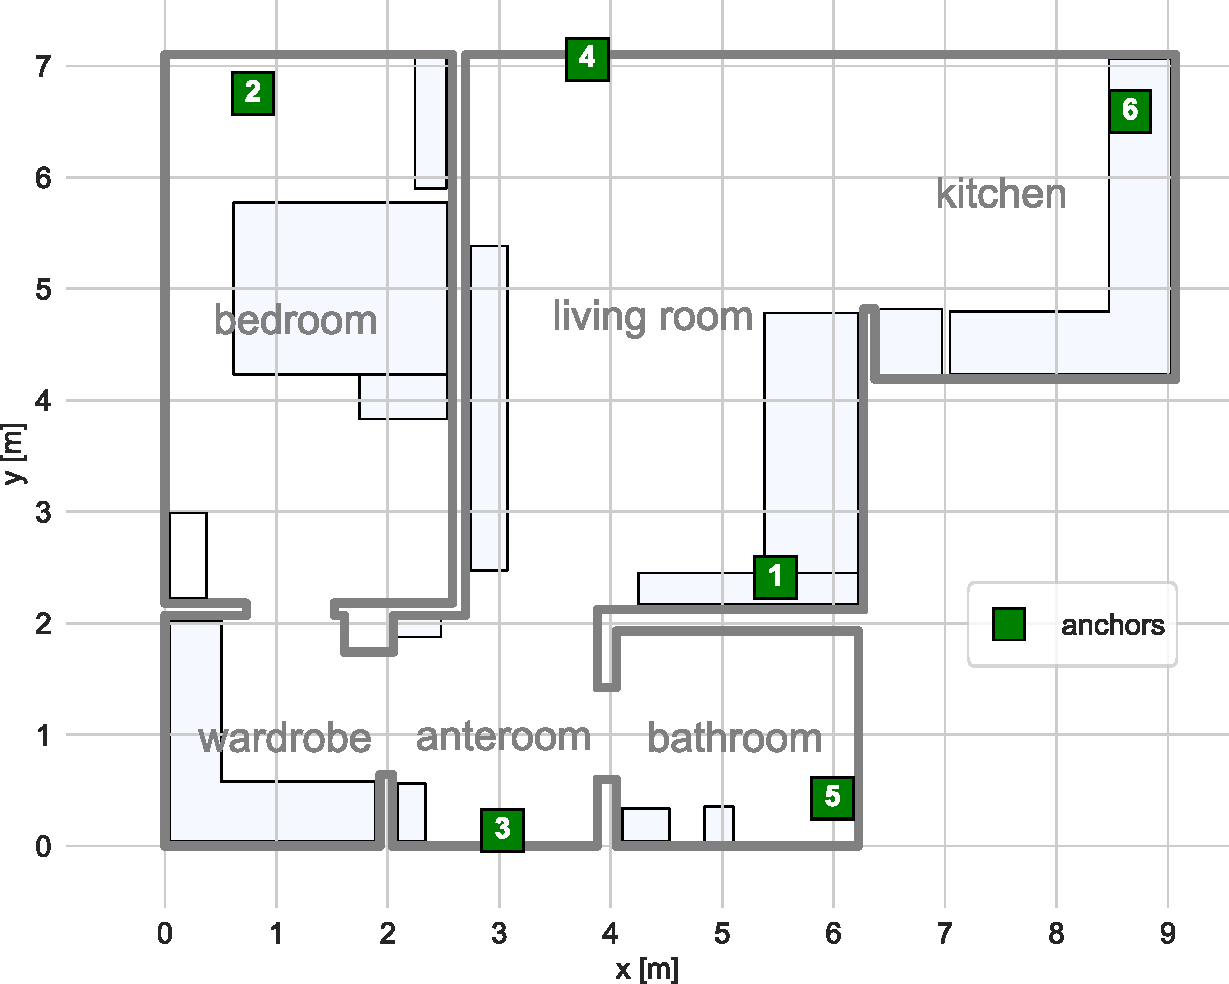
\includegraphics[width=.7\columnwidth]{figs/layout}}
\caption{Measurement environment with measurement locations and significant objects obstructing the path between the devices marked.}
\label{plan}
\end{figure}

The system infrastructure used in the study comprised six anchors, distributed among the apartment. The layout layout of the walls and anchor locations are stored in \texttt{layout.csv} and \texttt{anchors.csv} files respectively.

The used anchors are equipped with two Laird BL652 modules with external antennas of perpendicular polarization. In the system, the tag transmits BLE packets five times per second in three advertisement channels. The anchors periodically switch the reception channels and measure the power of the received signals. The results from both modules are averaged and sent to a localization server, which stores them in a database for future processing. The measurement results were gathered using a robotic platform, which is presented in Fig.\ref{fig:robot}.

\begin{figure}[h]
\centering
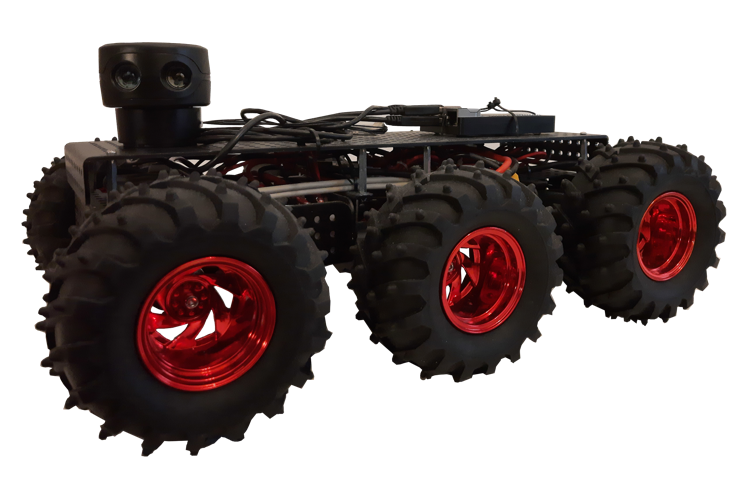
\includegraphics[width=0.5\columnwidth]{figs/robot}
\caption{\label{fig:robot}The mobile platform used in the study.}
\end{figure}

The platform was based on the Dagu Wild Thumper 6WD chassis and was controlled with a specially developed Python-based controller running on Raspberry Pi 4. The code for the controller and the PC applications used to gather the LiDAR results can be found at \cite{b2}.  The odometry measurements were performed by estimating the traveled distance and rotation angle through multiplying the elapsed time by the linear and rotation speed respectively.

The platform was equipped with a Scanse Sweep LiDAR, which is a discontinued 360 degree range sensor. During the study, the LiDAR was set to collect scans with a 2~Hz rate.

The system tag was attached at the middle the robot on a one meter long wooden pole, which placed it at the height of 1.3 m. Such height is close to a tag worn on a lanyard and ensures that low furniture pieces such as bed frames, couches or tables won't negatively impact the RSS measurement results.

The location of the calibration points are presented in Fig. \ref{fig:calibration}.

\begin{figure}[h]
\centering
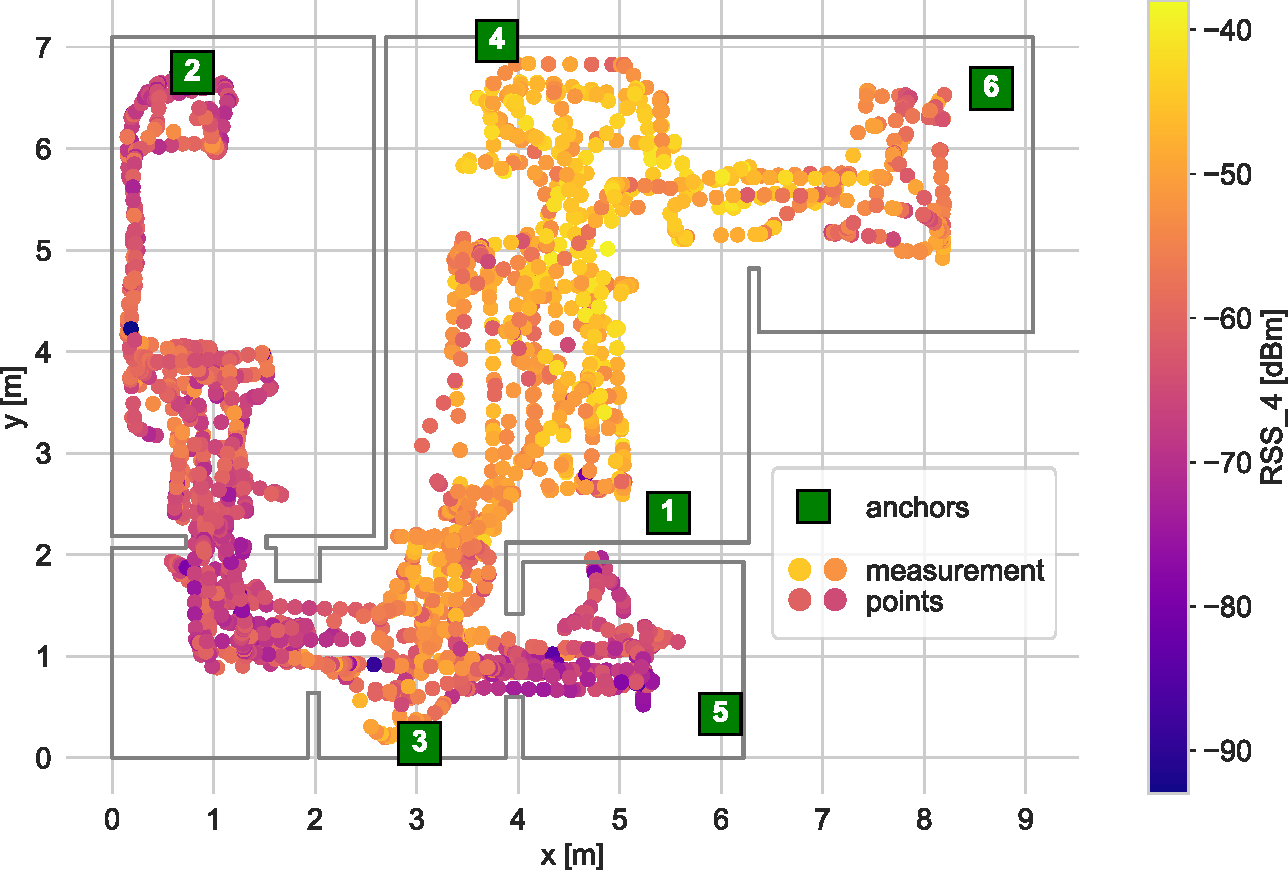
\includegraphics[width=.7\columnwidth]{figs/measurement_points}
\caption{\label{fig:calibration}Locations of calibration measurements. The colours of the points reflect the measured RSS value by anchor 4.}
\end{figure}

\section{Data processing}
The dataset contains preprocessed data. The SLAM measurements were used to create a radio map, which is a basis for positioning of the robotic platform during the calibration and test phases.

The processed calibration files contain DataFrames with robot locations and RSS values measured in them. The \texttt{calibration\_df.csv} file contains a DataFrame in which the robot locations are recalculated to take into account the displacement of the system tag from the LiDAR. The top-view schematic of the platform marking the respective sensors is presented in Fig. \ref{fig:displacement}.
\begin{figure}[h]
\centering
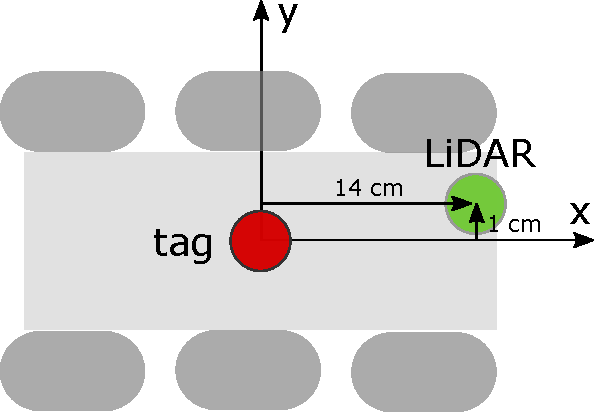
\includegraphics[width=.5\columnwidth]{figs/displacement}
\caption{\label{fig:displacement}The top-view schematic of the platform with Lidar and sensor displacements}
\end{figure}

\noindent
The robot test files were processed in the same manner as calibration files.
\color{red}
Please note that the identifiers of the anchors are changed after preprocessing from [3,4,5,8,10,11] to [1,2,3,4,5,6] respectively.
\color{black}


\section{Testing data}
The dataset requires two test measurements: one taken with a robot and one containing RSS measurements registered in a walking person localization. During the second experiment the person walked along the reference trajectory composed of straight lines. The coordinates of the trajectory vertices can be found in \texttt{tests/test\_walk\_df.csv} file. Each of the file's lines contains the coordinates of the line starting and ending points in the following order : $x_0$, $y_0$, $x_1$, $y_1$.


\section{Licence and attribution}

The dataset is licensed under \textit{Creative Commons Attribution 4.0 International} licence. The actual citation data can be found in the metadata on Zenodo or Readme file on Github.


\begin{thebibliography}{00} 
\bibitem{b1} J. Kolakowski, V. Djaja-Josko, M. Kolakowski, and K. Broczek, “UWB/BLE Tracking System for Elderly People Monitoring,” Sensors, vol. 20, no. 6, p. 1574, Mar. 2020, doi: 10.3390/s20061574.
\bibitem{b2} Marcin Kolakowski, Simple Raspberry Pi, Python based controlled for a robotic platform. 2021. Accessed: Aug. 12, 2021. [Online]. Available: https://github.com/marckolak/wtController


\end{thebibliography}
\vspace{12pt}
\color{red}

\end{document}
